\subsection{Future work \label{sec:Fut2}}

\subsubsection{HSL analogue derivatives}

A selection head groups which could be used in future conjugates are shown in \ref{fgr:fut_heads}. These have all been shown to modulate HSL-mediated quorum sensing as part of acyl-HSLs\cite{Smith2003a,Welch2005,Ishida2007,Olsen2002,Smith2003,Hodgkinson2012a,Marsden2010}. The most obvious targets are the cyclopentanone derivatives, as this could be synthesised from the alcohols above. The aniline, pyridine, quinoline and cyclopentyl amine head groups are commercially available and hence derivatives of these could be easily obtained. The 3- and 4-substituted HSL analogues require synthesis, but a convenient route has been devised\cite{Olsen2002}.

\begin{figure}[H]
	\begin{center}
		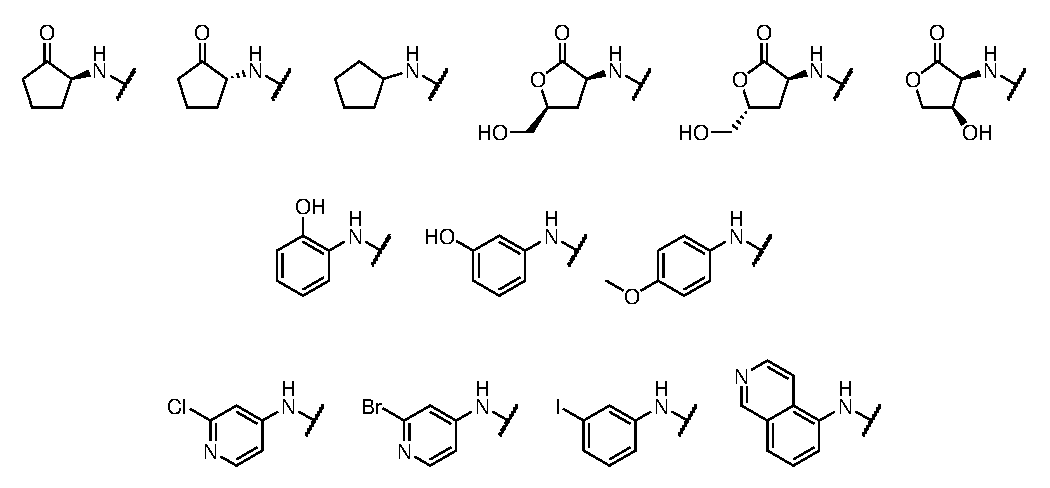
\includegraphics[scale=1]{fut_heads}
		\caption{HSL analogue head groups for use in future conjugates.
		\label{fgr:fut_heads}}
	\end{center}
\end{figure}

\todo{HL4CipMe}

\subsubsection{Biology}